\documentclass[14pt]{extbook}
\usepackage{multicol, enumerate, enumitem, hyperref, color, soul, setspace, parskip, fancyhdr} %General Packages
\usepackage{amssymb, amsthm, amsmath, bbm, latexsym, units, mathtools} %Math Packages
\everymath{\displaystyle} %All math in Display Style
% Packages with additional options
\usepackage[headsep=0.5cm,headheight=12pt, left=1 in,right= 1 in,top= 1 in,bottom= 1 in]{geometry}
\usepackage[usenames,dvipsnames]{xcolor}
\usepackage{dashrule}  % Package to use the command below to create lines between items
\newcommand{\litem}[1]{\item#1\hspace*{-1cm}\rule{\textwidth}{0.4pt}}
\pagestyle{fancy}
\lhead{Makeup Progress Quiz -1}
\chead{}
\rhead{Version C}
\lfoot{7547-2949}
\cfoot{}
\rfoot{Fall 2020}
\begin{document}

\begin{enumerate}
\litem{
Solve the linear equation below. Then, choose the interval that contains the solution.\[ \frac{5x -3}{4} - \frac{3x + 4}{2} = \frac{3x -3}{7} \]\begin{enumerate}[label=\Alph*.]
\item \( x \in [0.8, 2.9] \)
\item \( x \in [-2.6, -2] \)
\item \( x \in [-3.6, -2.8] \)
\item \( x \in [-6.1, -5.5] \)
\item \( \text{There are no real solutions.} \)

\end{enumerate} }
\litem{
Find the equation of the line described below. Write the linear equation as $ y=mx+b $ and choose the intervals that contain $m$ and $b$.\[ \text{Parallel to } 4 x - 9 y = 10 \text{ and passing through the point } (9, -9). \]\begin{enumerate}[label=\Alph*.]
\item \( m \in [-0.22, 0.84] \hspace*{3mm} b \in [-15, -11] \)
\item \( m \in [-0.49, -0.38] \hspace*{3mm} b \in [-7, -3] \)
\item \( m \in [-0.22, 0.84] \hspace*{3mm} b \in [10, 20] \)
\item \( m \in [-0.22, 0.84] \hspace*{3mm} b \in [-22, -17] \)
\item \( m \in [1.83, 2.83] \hspace*{3mm} b \in [-15, -11] \)

\end{enumerate} }
\litem{
Find the equation of the line described below. Write the linear equation as $ y=mx+b $ and choose the intervals that contain $m$ and $b$.\[ \text{Parallel to } 7 x - 6 y = 8 \text{ and passing through the point } (5, 5). \]\begin{enumerate}[label=\Alph*.]
\item \( m \in [1.07, 2.11] \hspace*{3mm} b \in [-1.02, -0.81] \)
\item \( m \in [1.07, 2.11] \hspace*{3mm} b \in [-0.01, 0.67] \)
\item \( m \in [-1.66, -0.24] \hspace*{3mm} b \in [10.67, 11.11] \)
\item \( m \in [1.07, 2.11] \hspace*{3mm} b \in [0.42, 1.28] \)
\item \( m \in [0.22, 1.15] \hspace*{3mm} b \in [-1.02, -0.81] \)

\end{enumerate} }
\litem{
Solve the linear equation below. Then, choose the interval that contains the solution.\[ \frac{-4x -5}{5} - \frac{7x + 7}{4} = \frac{-4x -3}{3} \]\begin{enumerate}[label=\Alph*.]
\item \( x \in [-0.25, 0.75] \)
\item \( x \in [-7.4, -4.4] \)
\item \( x \in [0.44, 3.44] \)
\item \( x \in [-1.44, -0.44] \)
\item \( \text{There are no real solutions.} \)

\end{enumerate} }
\litem{
Write the equation of the line in the graph below in Standard form $Ax+By=C$. Then, choose the intervals that contain $A, B, \text{ and } C$.
\begin{center}
    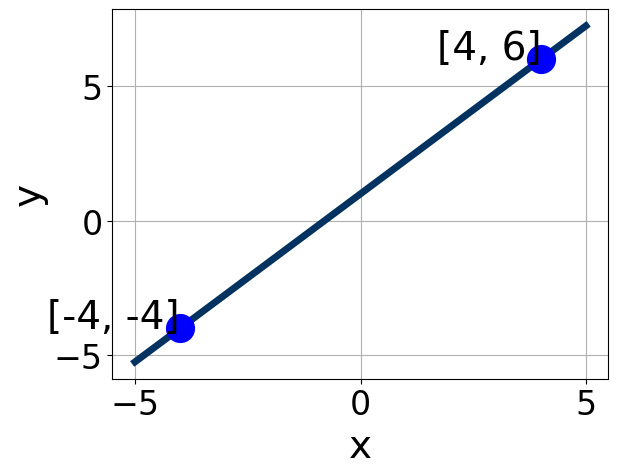
\includegraphics[width=0.5\textwidth]{../Figures/linearGraphToStandardCopyC.png}
\end{center}
\begin{enumerate}[label=\Alph*.]
\item \( A \in [4.5, 7.5], \hspace{3mm} B \in [2.3, 6.8], \text{ and } \hspace{3mm} C \in [3.86, 4.37] \)
\item \( A \in [-1.4, -0.2], \hspace{3mm} B \in [-2.7, -0.9], \text{ and } \hspace{3mm} C \in [-1.9, -0.32] \)
\item \( A \in [4.5, 7.5], \hspace{3mm} B \in [-7.3, -2.8], \text{ and } \hspace{3mm} C \in [-4.04, -3.4] \)
\item \( A \in [-1.4, -0.2], \hspace{3mm} B \in [0.2, 1.7], \text{ and } \hspace{3mm} C \in [-0.78, 1.88] \)
\item \( A \in [-5.8, -3], \hspace{3mm} B \in [2.3, 6.8], \text{ and } \hspace{3mm} C \in [3.86, 4.37] \)

\end{enumerate} }
\litem{
Solve the equation below. Then, choose the interval that contains the solution.\[ -6(8x -3) = -5(-18x -14) \]\begin{enumerate}[label=\Alph*.]
\item \( x \in [-1.08, -0.55] \)
\item \( x \in [-0.45, 0.28] \)
\item \( x \in [0.48, 1.05] \)
\item \( x \in [-2.3, -1.86] \)
\item \( \text{There are no real solutions.} \)

\end{enumerate} }
\litem{
Solve the equation below. Then, choose the interval that contains the solution.\[ -6(-15x + 12) = -17(-2x + 8) \]\begin{enumerate}[label=\Alph*.]
\item \( x \in [-1.3, 0.2] \)
\item \( x \in [0.2, 3.1] \)
\item \( x \in [2.2, 4.2] \)
\item \( x \in [-5.1, -2.3] \)
\item \( \text{There are no real solutions.} \)

\end{enumerate} }
\litem{
First, find the equation of the line containing the two points below. Then, write the equation as $ y=mx+b $ and choose the intervals that contain $m$ and $b$.\[ (6, -6) \text{ and } (5, -4) \]\begin{enumerate}[label=\Alph*.]
\item \( m \in [-4.1, 1.9] \hspace*{3mm} b \in [-12.96, -10.99] \)
\item \( m \in [-4.1, 1.9] \hspace*{3mm} b \in [5.73, 6.92] \)
\item \( m \in [-4.1, 1.9] \hspace*{3mm} b \in [-9.65, -7.79] \)
\item \( m \in [-4.1, 1.9] \hspace*{3mm} b \in [-6.63, -5.62] \)
\item \( m \in [-0.4, 4.6] \hspace*{3mm} b \in [-15.4, -13.76] \)

\end{enumerate} }
\litem{
First, find the equation of the line containing the two points below. Then, write the equation as $ y=mx+b $ and choose the intervals that contain $m$ and $b$.\[ (2, 4) \text{ and } (3, 3) \]\begin{enumerate}[label=\Alph*.]
\item \( m \in [0.89, 1.2] \hspace*{3mm} b \in [0, 1] \)
\item \( m \in [-2.15, -0.98] \hspace*{3mm} b \in [0, 1] \)
\item \( m \in [-2.15, -0.98] \hspace*{3mm} b \in [5, 9] \)
\item \( m \in [-2.15, -0.98] \hspace*{3mm} b \in [-7, -3] \)
\item \( m \in [-2.15, -0.98] \hspace*{3mm} b \in [1, 3] \)

\end{enumerate} }
\litem{
Write the equation of the line in the graph below in Standard form $Ax+By=C$. Then, choose the intervals that contain $A, B, \text{ and } C$.
\begin{center}
    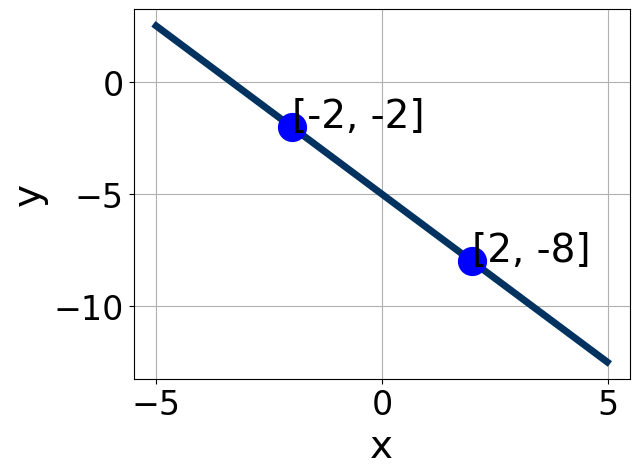
\includegraphics[width=0.5\textwidth]{../Figures/linearGraphToStandardC.png}
\end{center}
\begin{enumerate}[label=\Alph*.]
\item \( A \in [2.67, 3.12], \hspace{3mm} B \in [1.33, 2.03], \text{ and } \hspace{3mm} C \in [-10, -8] \)
\item \( A \in [2.67, 3.12], \hspace{3mm} B \in [-2.74, -1.88], \text{ and } \hspace{3mm} C \in [9, 13] \)
\item \( A \in [1.2, 1.56], \hspace{3mm} B \in [-1.35, -0.53], \text{ and } \hspace{3mm} C \in [4, 6] \)
\item \( A \in [1.2, 1.56], \hspace{3mm} B \in [0.95, 1.59], \text{ and } \hspace{3mm} C \in [-7, -4] \)
\item \( A \in [-4.49, -2.95], \hspace{3mm} B \in [-2.74, -1.88], \text{ and } \hspace{3mm} C \in [9, 13] \)

\end{enumerate} }
\end{enumerate}

\end{document}